\documentclass[11pt]{article}
\usepackage[margin=1in]{geometry}
\usepackage{amsmath,amssymb}
\usepackage{graphicx}
\usepackage{booktabs}
\usepackage{xcolor}
\usepackage{listings}
\usepackage{hyperref}
\usepackage[T1]{fontenc}
\usepackage{lmodern}

\lstset{basicstyle=\ttfamily\small, breaklines=true, columns=fullflexible, frame=single, upquote=true}
\newcommand{\TBD}[1]{\textcolor{red}{[TBD: #1]}}

\title{Assignment 2: Transformer\\\large INFO7375 Semantic Intelligence in LLM, Fall 2026}
\author{Fufan Lu (lu.fu@northeastern.edu)}
\date{}

\begin{document}
\maketitle

%======================================================================
\section*{Problem 1: Byte-Pair Encoding (BPE) Tokenizer}

\subsection*{Q1.1 A. Failures of a public tokenizer}
All three tests use \texttt{google-bert/bert-base-cased} (WordPiece); the code is in \texttt{tests/test\_tokenizer.py} and all three assertions pass.
\begin{itemize}
  \item \textbf{Not injective.} \texttt{"I love }\textit{<robot emoji U+1F916>}\texttt{"} and \texttt{"I love }\textit{<parrot emoji U+1F99C>}\texttt{"} both encode to \texttt{[146, 1567, 100]}, because every character outside the WordPiece vocabulary becomes the same \texttt{[UNK]} token (id 100). Two different strings therefore share one token sequence.
  \item \textbf{Not invertible.} The tokenizer splits punctuation into its own token and \texttt{decode} joins tokens with spaces, so \texttt{"don't stop"} comes back as \texttt{"don ' t stop"}. The original string cannot be recovered from its tokens.
  \item \textbf{Does not preserve concatenation.} \texttt{tokenize("token"+"ization")} is \texttt{[token, \#\#ization]}, while \texttt{tokenize("token") + tokenize("ization")} is \texttt{[token] + [i, \#\#zation]}. Inside a word WordPiece uses \texttt{\#\#} continuation pieces, which differ from the pieces used at the start of a word.
\end{itemize}

\subsection*{Q1.1 B. Why non-trivial tokenizers cannot preserve concatenation}
Suppose a tokenizer preserves concatenation, and let $t \in \mathcal{V}$ be any multi-character token, $t = xy$ with $x, y$ non-empty strings. Then $\text{tokenize}(t) = \text{tokenize}(x) + \text{tokenize}(y)$, and since both parts are non-empty token sequences, $t$ is tokenized into at least two tokens: the single token $t$ can never be emitted. Applying the same argument to every string shows that $\text{tokenize}(c_1 \cdots c_n) = \text{tokenize}(c_1) + \cdots + \text{tokenize}(c_n)$, i.e.\ the tokenizer is completely determined by how it maps individual characters, so every multi-character token in the vocabulary is unreachable and the tokenizer is equivalent to the trivial one. Put differently, the whole point of merging (e.g.\ \texttt{a}, \texttt{b} $\to$ \texttt{ab}) is to tokenize a string differently depending on its neighbours, and concatenation creates exactly such new neighbours at the boundary.

\subsection*{Q1.2 BPE implementation}
\texttt{ASCIIBPETokenizer.merge}, \texttt{encode} and \texttt{decode} are implemented in \texttt{src/tokenizer/bpe.py}; all \texttt{test\_*\_merge}, \texttt{test\_encode} and \texttt{test\_decode} tests pass. \texttt{encode} replays the learned merges in the order they were learned; one pass suffices because a later merge never creates a new occurrence of an earlier bigram.

\subsection*{Q1.3 Learned tokens of the English tokenizer}
\textbf{A.} The longest learned token is \texttt{"\textbackslash n\textbackslash nReferences"} (12 bytes), followed by its intermediate pieces \texttt{"ferences"} and \texttt{"feren"} and then frequent words such as \texttt{" which"}, \texttt{" with"}, \texttt{" from"}, \texttt{" that"}. This shows the training data is Wikipedia: nearly every article ends with a \emph{References} section, so that boilerplate string was frequent enough to be merged into a single token.

\textbf{B.} BPE merges whatever strings are most frequent in the training corpus, so a sensitive string that is repeated often (a name, email address, phone number or API key) can become a token, and publishing the vocabulary then reveals that the string was in the private data. The merge order also leaks relative frequencies, which can be used to infer the composition of the training data.

\subsection*{Q1.4 English vs.\ Thai}
\textbf{A.} Yes: the English document uses 119 tokens while its Thai translation uses 636 (5.3$\times$), although the two strings have a similar number of characters (249 vs.\ 239). The tokenizer was trained only on English, so it learned no merges for Thai; every Thai character takes 3 bytes in UTF-8, and the 659 bytes end up as 636 tokens, almost one token per byte.

\textbf{B.} Users of low-resource languages pay more for the same content (APIs bill per token), fit less text into the context window, wait longer for generation, and usually get worse model quality because each token carries less information, which is a systematic unfairness between languages.

%======================================================================
\section*{Problem 2: Implementing a Transformer}

\subsection*{Q2.1 Weight tying}
Weight tying (Press \& Wolf, 2017) uses one matrix both as the input embedding and as the output projection, so the logit of token $v$ is the dot product of the final hidden state with $v$'s input embedding. This removes the separate $V \times d$ output matrix, which is a large share of a small model's parameters (here $V = 50257$), and acts as a regularizer. The paper shows that the tied embedding, trained through both its input and output roles, gives lower perplexity.

\subsection*{Q2.2 Logits with weight tying}
\begin{lstlisting}[language=Python]
logits = h @ E.T   # (b, s, d) @ (d, v) -> (b, s, v); same as torch.einsum("bsd,vd->bsv", h, E)
\end{lstlisting}

\subsection*{Q2.3 Implementation}
\texttt{MultiHeadAttention}, \texttt{FeedForward}, \texttt{DecoderBlock} and \texttt{DecoderLM} are implemented in \texttt{src/lm/model.py} without loops over matrix operations; all tests in \texttt{tests/test\_model.py} pass (the CUDA-only test is skipped on a machine without CUDA). Design choices: pre-LN blocks (GPT-2 style, matching the final \texttt{LayerNorm} in \texttt{DecoderLM}); masked logits are filled with the dtype minimum rather than $-\infty$ and the masked weights are zeroed after the softmax, so rows that are entirely padding output zeros instead of NaN; position ids are \texttt{cumsum(mask) - 1} so left padding does not shift positions; logits use weight tying.

%======================================================================
\section*{Problem 3: Training the Transformer}

\subsection*{Q3.1 Implementation}
All functions in \texttt{src/lm/train.py} are implemented and all tests in \texttt{tests/test\_train.py} pass, including \texttt{test\_train\_sanity\_check} (validation loss $2.080 \approx \log 8$ in five repeated runs, i.e.\ the model does not see the token it predicts). The training loop clips the gradient norm at 1.0 before each optimizer step.

\subsection*{Q3.2 Cosine annealing with warmup}
\textbf{A.}
\[
\text{lr}(t) =
\begin{cases}
\text{lr}_{max}\,\dfrac{t}{a}, & 0 \le t < a \quad \text{(warmup)}\\[2ex]
\text{lr}_{min} + \dfrac{1}{2}\left(\text{lr}_{max} - \text{lr}_{min}\right)\left(1 + \cos\!\left(\pi\,\dfrac{t-a}{b-a}\right)\right), & a \le t < b \quad \text{(annealing)}\\[2ex]
\text{lr}_{min}, & t \ge b
\end{cases}
\]

\textbf{B.} Large steps early make fast progress while the model is far from a good solution, and steadily smaller steps later let the optimizer settle into a low-loss region instead of bouncing around it, so cosine annealing usually reaches a lower final loss than a constant learning rate; the schedule is smooth with no decay milestones to tune, and the short warmup avoids unstable first updates while Adam's moment estimates are still poor.

\subsection*{Q3.3 GPT-tiny}
\textbf{A.} With the provided \texttt{GPT-tiny.yaml} (2000 steps, $8.13\times10^{13}$ FLOPs) the validation loss is \textbf{7.052} (perplexity 1155).

\textbf{B.} The provided 2000 steps are far from saturation: the loss is still falling when the schedule ends. To find where it saturates I trained the same configuration for longer (only \texttt{num\_training\_steps} changed):
\begin{center}
\begin{tabular}{rrrr}
\toprule
steps & tokens & val loss & val PPL \\
\midrule
2{,}000 & 8.2M & 7.052 & 1155 \\
8{,}000 & 32.8M & 6.269 & 528 \\
20{,}000 & 81.9M & 6.046 & 422 \\
\bottomrule
\end{tabular}
\end{center}
The training loss flattens after roughly \textbf{10{,}000 steps} ($\approx$40M tokens): it is about 6.35 at step 10k and only about 6.3 at step 20k (Figure~\ref{fig:tiny-lengths}), while quadrupling the steps from 2k to 8k had gained 0.78 nats of validation loss. So GPT-tiny should be trained for about 10k steps; beyond that its 2M parameters (mostly the embedding, $d=32$) leave little to gain.

\textbf{C.} Training curve of the provided GPT-tiny run (logged to Weights \& Biases as \texttt{train-loss}; the dashed line is the learning rate):
\begin{center}
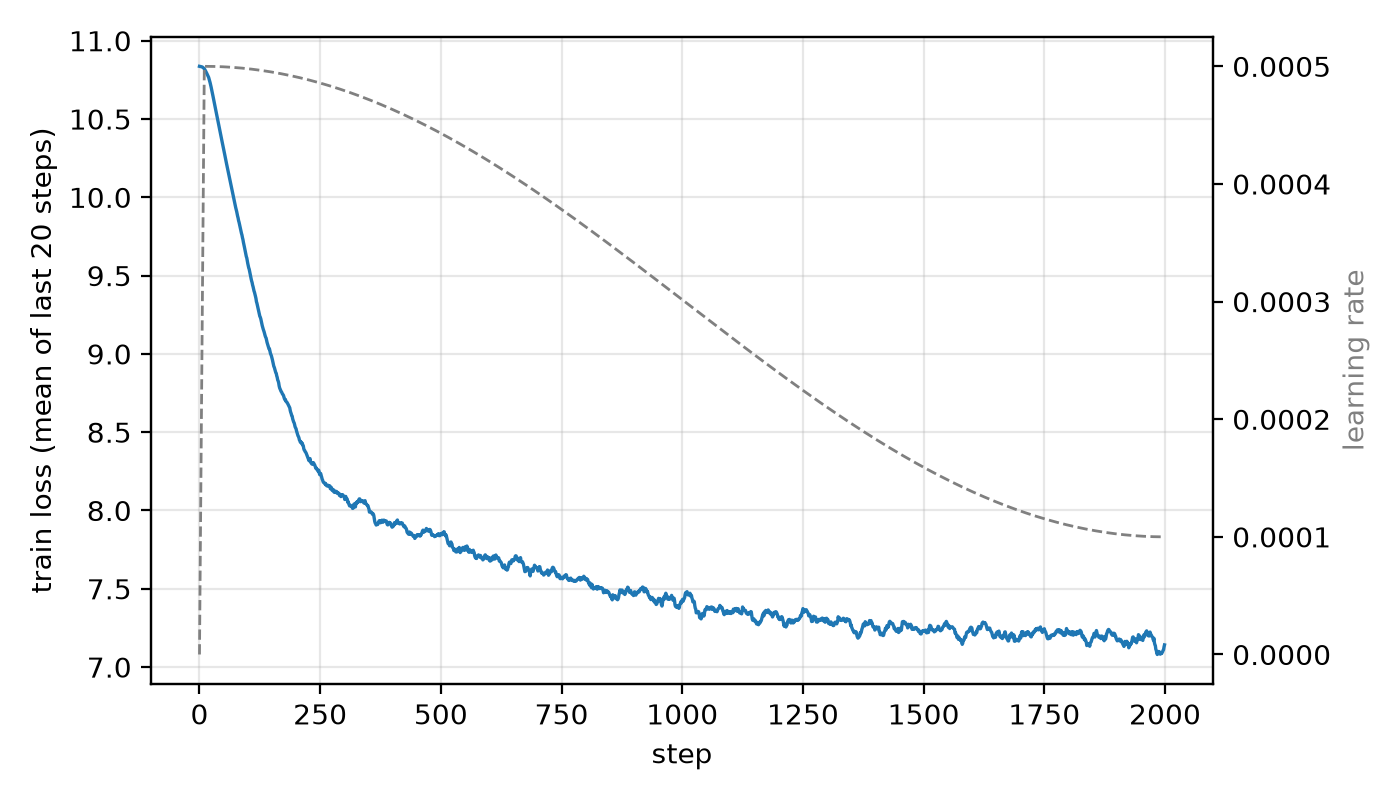
\includegraphics[width=0.8\linewidth]{figures/gpt_tiny_2000.png}
\end{center}
\begin{figure}[h]
\centering
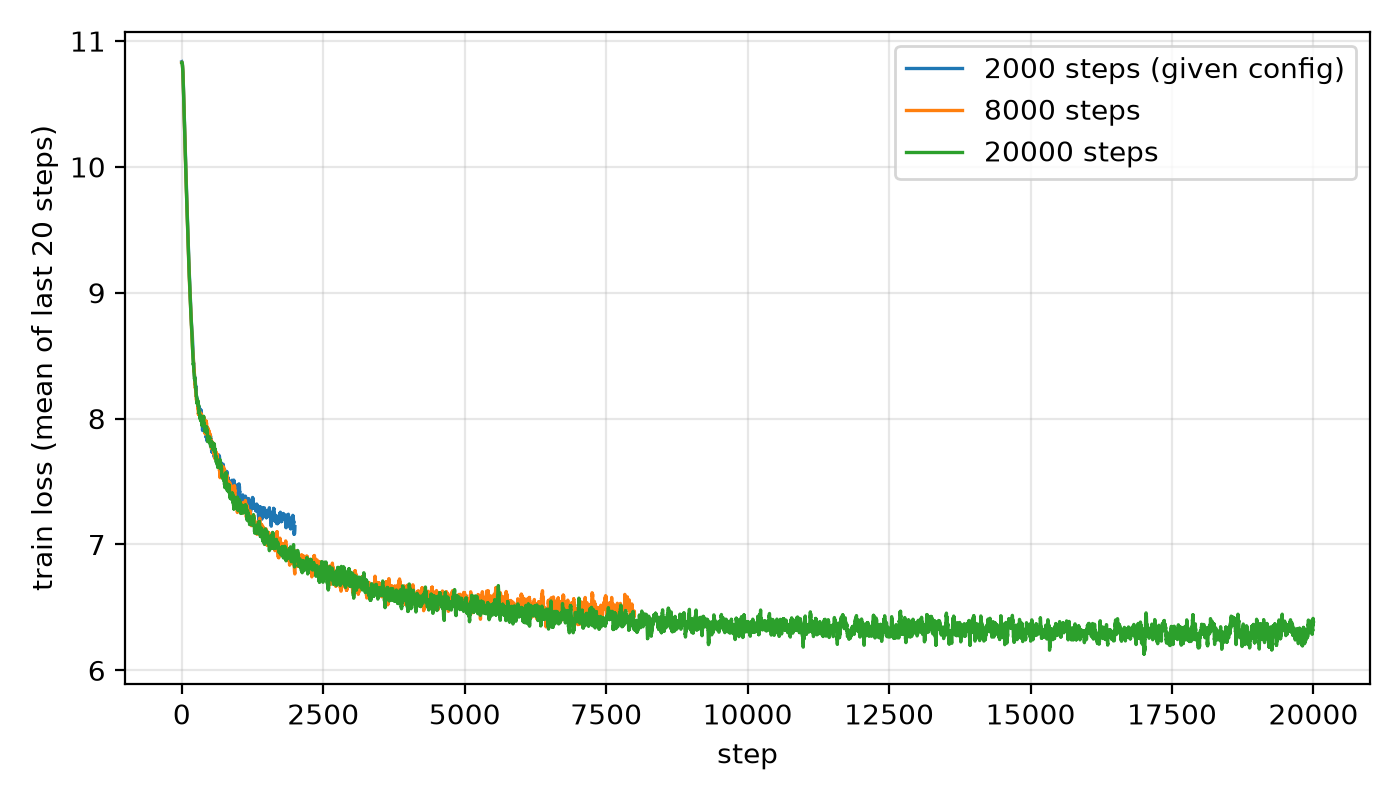
\includegraphics[width=0.8\linewidth]{figures/gpt_tiny_lengths.png}
\caption{GPT-tiny trained for 2k, 8k and 20k steps (each with its own cosine schedule).}
\label{fig:tiny-lengths}
\end{figure}

\subsection*{Q3.4 Hyperparameter search under $10^{15}$ FLOPs}
\textbf{A. Procedure.} Every run uses at most $10^{15}$ training FLOPs as counted by \texttt{train.py}; for each configuration I set \texttt{num\_training\_steps} $=\lfloor 10^{15} / (\text{FLOPs per token} \times \text{batch} \times \text{seq\_len}) \rfloor$. Because Q3.5 keeps the model hyperparameters fixed and must reach perplexity below 50 with $10^{17}$ FLOPs and a checkpoint under 100MB, I limited the search to models that can plausibly do that: with the 50257-token vocabulary, the tied embedding alone holds $50257\,d$ parameters, so an fp32 checkpoint under 100MB requires $d \le 320$; I therefore considered $d \in \{256, 320\}$ with 6--12 layers (17--24M parameters), keeping \texttt{n\_positions} $=$ \texttt{seq\_len} $=128$. The search had two rounds with selection rules fixed in advance (validation perplexity on the held-out 5M-token split): round 1 kept the model fixed (d256, 8 layers, 8 heads) and varied the training recipe; round 2 applied the best recipe to a deeper (12 layers) and a wider ($d=320$, 6 layers, head size 64) model. All five runs used one NVIDIA H200 with bf16 autocast. As a check, configuration A was also trained on a V100 in fp32 and reached perplexity 407.2 (vs.\ 402.6), so the numeric precision barely matters.

\textbf{B. Results.}
\begin{center}
\small
\begin{tabular}{llrrrrr}
\toprule
 & what changed & params & steps & tokens & val loss & val PPL \\
\midrule
A & d256/L8/H8; GPT-tiny recipe: lr $5\mathrm{e}{-4}\!\to\!1\mathrm{e}{-4}$, warmup 10, batch 32 & 19.2M & 2061 & 8.4M & 5.998 & 402.6 \\
\textbf{B} & \textbf{as A, lr $2\mathrm{e}{-3}\!\to\!2\mathrm{e}{-4}$, warmup 100} & 19.2M & 2061 & 8.4M & \textbf{5.845} & \textbf{345.4} \\
C & as B, batch 16 (twice the updates, same tokens) & 19.2M & 4122 & 8.4M & 5.949 & 383.4 \\
D & as B, 12 layers (deeper) & 22.4M & 1756 & 7.2M & 5.952 & 384.7 \\
E & as B, $d=320$, 6 layers, 5 heads (wider) & 23.5M & 1694 & 6.9M & 5.914 & 370.3 \\
\bottomrule
\end{tabular}
\end{center}
The learning rate mattered most: raising the peak learning rate from $5\times10^{-4}$ to $2\times10^{-3}$ lowered perplexity from 402.6 to 345.4. Halving the batch size to get twice as many updates hurt (383.4), presumably because the noisier gradients at this learning rate outweigh the extra steps. Under a fixed FLOP budget, the larger models see fewer tokens (7.2M and 6.9M instead of 8.4M) and end up worse even though the wider model E learns fastest per token early on (Figure~\ref{fig:hparam}); at $10^{15}$ FLOPs the budget is too small for the extra capacity to pay off. The best configuration is \textbf{B}: $d=256$, 8 layers, 8 heads, 128 positions (19.2M parameters, 76.9MB), peak learning rate $2\times10^{-3}$.
\begin{figure}[h]
\centering
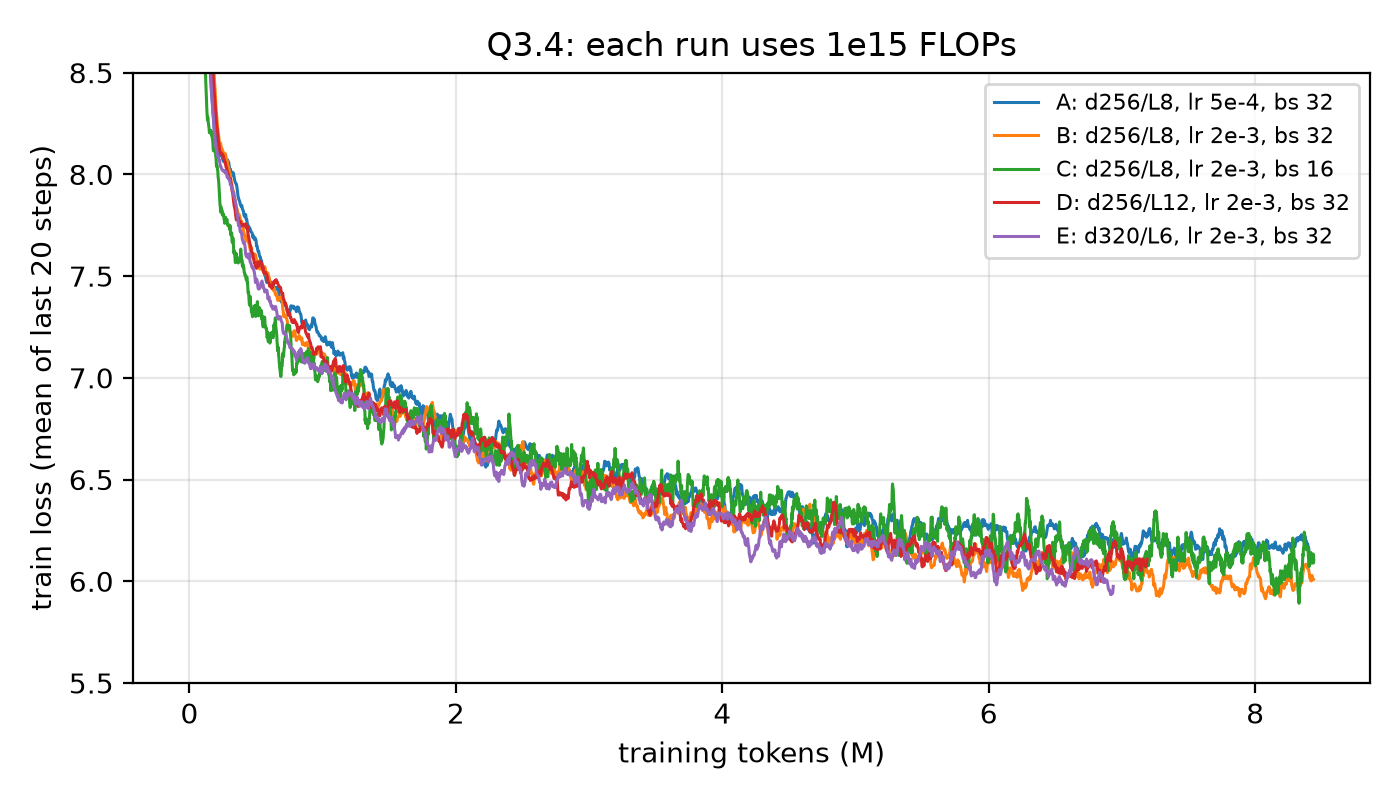
\includegraphics[width=0.8\linewidth]{figures/hparam_curves.png}
\caption{Training loss of the five configurations against training tokens.}
\label{fig:hparam}
\end{figure}

\textbf{C. Final configuration} (\texttt{configs/hparam/B\_d256L8\_lr2e-3.yaml}):
\lstinputlisting{../configs/hparam/B_d256L8_lr2e-3.yaml}

\subsection*{Q3.5 Final model}
The final model keeps the model hyperparameters of configuration B ($d=256$, 8 heads, 128 positions, 8 layers; 19.2M parameters) and only changes the training hyperparameters to use $\approx 10^{17}$ FLOPs ($1.00\times10^{17}$ as reported by \texttt{train.py}): batch size 256 $\times$ 128 tokens, 25{,}764 steps ($\approx$844M tokens, about 1.6 passes over the 520M training tokens), 515 warmup steps (2\%), peak learning rate $2\times10^{-3}$ annealed to $2\times10^{-4}$. A larger batch than in Q3.4 keeps the GPU busy (39 TFLOPS on one H200, 45 minutes).

\begin{center}
\begin{tabular}{lr}
\toprule
Final validation loss & \textbf{3.596} \\
Final validation perplexity & \textbf{36.46} \\
Checkpoint (\texttt{model.pt}) & 76.9MB \\
\bottomrule
\end{tabular}
\end{center}
Configuration (\texttt{config.yaml}, submitted with \texttt{model.pt}):
\lstinputlisting{../outputs/final/config.yaml}

%======================================================================
\section*{Problem 4: Text Generation \& Perplexity Analysis}

\subsection*{Q4.1 Implementation}
\texttt{softmax\_with\_temperature} and a batched \texttt{generate} (left padding with \texttt{eot\_token}, attention mask 0 on padding) are implemented in \texttt{src/lm/generate.py}; \texttt{test\_generate.py} passes. The reported perplexity is computed over the generated tokens only: $\exp$ of the mean negative log-likelihood the model assigns (at temperature 1) to each sampled token given everything before it.

\subsection*{Q4.2 Generations}
\textbf{A. Prefixes and settings.} I used three of the provided prefixes (\texttt{data/prefixes.jsonl}: a news-magazine paragraph, a 19th-century biography and a popular-science news lead):
\begin{enumerate}
  \item Hammer a tube called a spile into the bark of a maple tree and its translucent yellow sap will start flowing out; the tree has been tapped (pictured). This gloop drips from some 55m Canadian maple trees today, raw material for the tangy golden syrup which is one of the country's proudest exports.
  \item CHARLES H. MEISNER, one of the prosperous and highly-esteemed business men of Birnamwood, Shawano county, was born in Newton township, Manitowoc Co., Wis., February 14, 1860, and is a son of Frederick and Magarette (Steltzer) Meisner, both natives of Germany.
  \item EVER WONDER WHY SOME PEOPLE CAN WORK NIGHTS AND SLEEP EASILY DURING THE DAY? A new study from Tiina Pauno, a professor at the University of Helsinki, Finland found that many night workers actually have a variant in the genetic code that makes them less influenced by Melatonin and hence the circadian rhythm.
\end{enumerate}

Both models generated \texttt{max\_new\_tokens} $=48$ tokens per prefix at temperatures $T \in \{0.01, 0.5, 1.0\}$ (our model with \texttt{src/lm/generate.py} and the Q3.5 checkpoint; Pythia-1.4B with \texttt{src/lm/use\_pythia.py}, which samples with \texttt{do\_sample=True}). $T=0.01$ stands in for ``near zero'' because Hugging Face sampling requires $T>0$. Generations, prefix by prefix:
{\small \paragraph{Our model (final checkpoint from Q3.5)}
\noindent\textit{Prefix 1.}\begin{itemize}
  \item $T=0.01$: \textcolor{blue!60!black}{The tree is a small, small, small, small, small, small, small, small, small, small, small, small, small, small, small, small, small, small, small, small, small, small}
  \item $T=0.5$: \textcolor{blue!60!black}{The color is a plumber, but it is a great choice for the grain and the taste. It was a great time to see the best of the very best of the new and the most brilliant ingredients to have. The fruit}
  \item $T=1.0$: \textcolor{blue!60!black}{This structure is unplugged and makes it HUD at least the most popular ever-designed magazine around the world before. ANoticeless ascended rather than even writing a second and gieser guild to buy groceries into the duckwall to invest}
\end{itemize}
\noindent\textit{Prefix 2.}\begin{itemize}
  \item $T=0.01$: \textcolor{blue!60!black}{The first of the first of the first of the first of the first of the first of the first of the first of the first of the first of the first of the first of the first of the first of the first of the first}
  \item $T=0.5$: \textcolor{blue!60!black}{The company also has been considered as a brand new company. The company has been considered as a brand new company, a company founded in 1986, and is a member of the company. The company has been considered as a brand}
  \item $T=1.0$: \textcolor{blue!60!black}{/? Others from this site Reading to 6 Constitution Required: Since 2001, the literary community will be presented primarily from the original Xbox One Company in Virginia, the American Indian Book". (1) Obama Leader Essays to}
\end{itemize}
\noindent\textit{Prefix 3.}\begin{itemize}
  \item $T=0.01$: \textcolor{blue!60!black}{The study was conducted by the University of Helsinki, Finland, which was conducted by the University of Helsinki, Finland, and the University of Helsinki, Finland. The study was conducted by the University of Helsinki, Finland, and the University of}
  \item $T=0.5$: \textcolor{blue!60!black}{The study was conducted by a professor at the University of Helsinki, Finland, where she was an independent professor at the University of Helsinki, Finland. The study was conducted by a professor at the University of Helsinki, Finland, and was the}
  \item $T=1.0$: \textcolor{blue!60!black}{Read more about Johannes, who did not write this and booth possibly metabolic studies, which included Giendouke Leonard Baker in the research groups of the other studies written in an attempt to leverage the its ownurrence. Jones has gone into this}
\end{itemize}
\paragraph{Pythia-1.4B}
\noindent\textit{Prefix 1.}\begin{itemize}
  \item $T=0.01$: \textcolor{blue!60!black}{The sap is collected in the spring, when the maple trees are still green, and is then boiled down to make maple syrup. The sap is then collected in the fall, when the maple trees are already brown and the}
  \item $T=0.5$: \textcolor{blue!60!black}{The process of tapping maple trees is a complex one, involving a number of steps. The sap rises from the tree's trunk and runs down a tube into a wooden spile, which is then attached to a wooden handle.}
  \item $T=1.0$: \textcolor{blue!60!black}{TAP: What is maple syrup? A: It's the sticky, syrup-like sap dripping from the maple tree. B: It's one of Canada's top-ranking agricultural export products. TAP: How is it made (}
\end{itemize}
\noindent\textit{Prefix 2.}\begin{itemize}
  \item $T=0.01$: \textcolor{blue!60!black}{He was educated in the public schools of Manitowoc county, and at the age of eighteen years was employed as a clerk in the office of the county treasurer. He was married to Miss Mary E. (Hoffman) Me}
  \item $T=0.5$: \textcolor{blue!60!black}{He was educated in the public schools of Manitowoc county, and received his education in the public schools and private schools of Wisconsin. He was graduated from the University of Wisconsin at Madison, Wisconsin, in 1882, and from the law department}
  \item $T=1.0$: \textcolor{blue!60!black}{His father was born in Gau-Sachsen, Prussia, February 16, 1823, and is a native of Wernigerode. He graduated from the high school at Dresden, Germany, in 1851,}
\end{itemize}
\noindent\textit{Prefix 3.}\begin{itemize}
  \item $T=0.01$: \textcolor{blue!60!black}{The study, published in the journal Nature Communications, found that the variant is associated with a lower level of melatonin production. The researchers found that the variant is associated with a lower level of melatonin production.}
  \item $T=0.5$: \textcolor{blue!60!black}{Researchers analyzed the genetic makeup of more than 3,000 people who worked in factories, offices, and other places where there is a high risk of exposure to chemicals. They found that the genes for Melatonin production were more common}
  \item $T=1.0$: \textcolor{blue!60!black}{So do you need sleep and wake up often throughout the day? The answer is most likely no. But some people get used to doing that. They say things they would never say at work, or they go out and drink when}
\end{itemize}
}

Perplexities of the generated continuations (3 prefixes $\times$ 48 tokens) at each temperature. ``Self'' is each model's perplexity on its own continuations (temperature-1 probabilities of the sampled tokens given everything before them, as printed by \texttt{generate.py}); ``judged by Pythia'' scores the continuations with Pythia-1.4B as a common reference model (\texttt{scripts/score\_continuations.py}).
\begin{center}
\begin{tabular}{rrrr}
\toprule
$T$ & ours, self & Pythia, self (= judged by Pythia) & ours, judged by Pythia \\
\midrule
0.01 & 2.10 & 3.33 & 2.80 \\
0.5 & 7.21 & 3.49 & 16.55 \\
1.0 & 193.09 & 7.02 & 575.94 \\
\bottomrule
\end{tabular}
\end{center}

\textbf{B.} Near zero the softmax turns into an argmax, so decoding becomes greedy and deterministic: both models fall into loops (ours repeats ``small, small, small, \ldots'' and ``The first of the first of\ldots''; Pythia repeats ``the variant is associated with a lower level of melatonin''), and perplexity is very low. Near one the models sample from their full distribution, so the text is more varied and less repetitive but also less coherent, which for our small model means drifting into nonsense (perplexity 193).

\textbf{C.} At $T=0.01$ our model even scores a lower perplexity than Pythia (2.10, or 2.80 judged by Pythia, vs.\ 3.33), but only because its degenerate loops are trivially predictable, so a low perplexity does not mean better text. At $T=0.5$ and $1.0$, Pythia's continuations stay fluent and on topic while ours are grammatical but empty at 0.5 and incoherent at 1.0; Pythia finds our text 5--80$\times$ less likely than its own (16.55 vs.\ 3.49, 575.94 vs.\ 7.02). The gap comes from scale: Pythia-1.4B has about 70$\times$ more parameters, was trained on about 300B tokens of the Pile (vs.\ our 0.84B) with a 2048-token context (vs.\ 128), so its next-token distribution is much sharper, whereas ours (validation perplexity 36.5) spreads probability over many tokens that derail the text when sampled.

\subsection*{Q4.3 Perplexity under Pythia-1.4B}
\begin{center}
\begin{tabular}{lr}
\toprule
Document & PPL (Pythia-1.4B) \\
\midrule
Northeastern University Wikipedia paragraphs & 7.10 \\
\quad same text with every ``the''/``The'' removed (8 words) & 9.27 \\
Jabberwocky (original) & 1.58 \\
Jabberwocky mimic (nonsense words swapped) & 18.92 \\
\bottomrule
\end{tabular}
\end{center}
Each document was evaluated on its own (\texttt{-{}-batch\_size 1}), since \texttt{evaluate\_perplexity.py} pools all documents in a file into one number.

\textbf{A.} The Wikipedia paragraphs have perplexity 7.10, which rises to 9.27 after every ``the'' is removed. ``the'' is one of the easiest tokens to predict, and removing it also makes the text ungrammatical, so the words that follow (e.g.\ a noun the model expected to come after a determiner) become harder to predict, raising the average negative log-likelihood.

\textbf{B.} The original Jabberwocky has perplexity 1.58, while my mimic has 18.92. The original is a famous poem that almost certainly appears many times in Pythia's training data (\emph{Through the Looking-Glass} is in Project Gutenberg, which is part of the Pile, and the poem is quoted all over the web), so the model has essentially memorized it, nonsense words included; my invented words never appeared in training, so the model cannot recall them and can only predict the ordinary English around them.

My mimic poem (first stanza shown; every stanza swaps several nonsense words, the full text is in \texttt{data/ppl/jabberwocky\_mimic.jsonl}):
\begin{lstlisting}
'Twas frindle, and the plorky voats
      Did skirl and wumble in the drabe:
All flimty were the kittipoos,
      And the zome grackths outsnabe.
\end{lstlisting}

%======================================================================
\section*{Problem 5: Use of Generative AI}
\textbf{Q5.1.} Yes: Claude Code (Anthropic's coding agent).

\textbf{Q5.2.} I used Claude Code to read the assignment and starter code, implement the missing functions, run the tests, set up and launch the training jobs on the Explorer cluster, and draft the written answers, which I reviewed. Sample prompts: ``Look at this assignment and tell me how to do it.''; ``Go ahead and do it; you can use the school's GPU cluster.''

\textbf{Q5.3.} No other use.

\end{document}
